 \سؤال{مشاهده‌ی فایل سیستم \lr{/proc}}
 
 \begin{enumerate}
 	\item با استفاده از دستور \lr{cd}  وارد شاخه‌ی \lr{/proc} می‌شویم.
 	
 	\begin{code}
 		> cd /proc
 	\end{code}
 
 	\item به کمک دستور \lr{ls} فایل‌های موجود در این شاخه را مشاهده می‌کنیم.
 	
 	\begin{code}
 		> ls
 	\end{code}
 	
 	\item فایل‌های موجود به همراه \lr{Process ID}ها
 	
 		\begin{figure}[!hbpt]
 			\centering
 			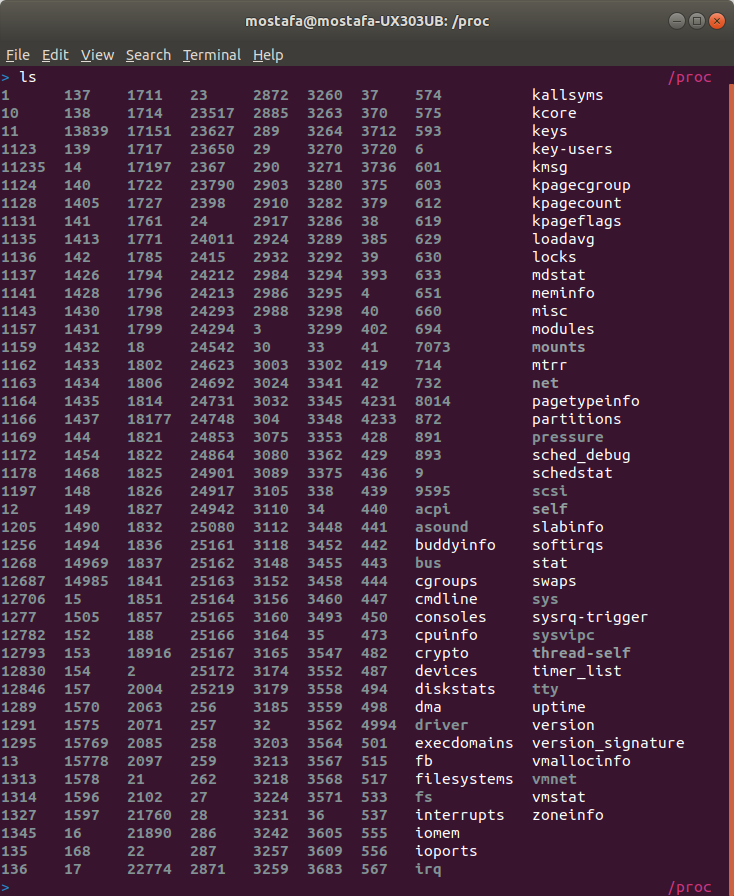
\includegraphics[scale=.35]{./img/1.png}
 			\caption{دستورهای سوال اول}
 		\end{figure}
\end{enumerate}

\newpage

\سؤال{مشاهده‌ی محتویات یک فایل در شاخه \lr{/proc}}

\begin{enumerate}
	\item محتوای فایل \lr{/proc/version}. 
	این فایل نام نسخه‌ی واقعی سیستم‌عامل را نشان نمی‌دهد، در عوض مشخصات مربوط به نسخه هسته‌ی لینوکس استفاده شده در توزیع و هم‌چنین نسخه‌ی کامپایلر \lr{GCC} که برای ساخت آن استفاده شده را نمایش می‌دهد.
	
	\begin{code}
		> cat version
		
		Linux version 5.4.0-42-generic (buildd@lgw01-amd64-023) (gcc version 7.5.0 		(Ubuntu
		
		 7.5.0-3ubuntu1~18.04)) \#46~18.04.1-Ubuntu SMP Fri Jul 10 07:21:24 UTC 2020
	\end{code}


	\item 
	
	
	\begin{itemize}
		\item \textbf{\lr{cmdline}}: در این فایل، پارامترهایی که سیستم هنگام \lr{boot} شدن از آن‌ها استفاده می‌کند را می‌توان بررسی کرد و هم‌چنین می‌توان دید که آیا شامل تغییرات است یا خیر.
		
		\item \textbf{cpuinfo}: نوع پردازنده و تعداد پردازنده‌های در حال اجرا را نمایش می‌دهد. 
		
		\item \textbf{diskstats}: آمارهای ورودی و خروجی مربوط به \lr{block devices} را نمایش می‌دهد.		
	\end{itemize}

	\item
	
	\item
\end{enumerate}

